\chapter{Introduction}
\label{the-introduction}
% This should cover the problem the thesis addresses, the aims and questions, the thesis structure, a summary of the main findings and a discussion on the thesis' contribution. It should prime the reader for what's about to come by providing an overview of what lies ahead.

% Establish your research territory by situating your research in a broader context. 
% Establish and justify your niche by describing why your research is needed. 
% Explain the significance of your research by describing how you conducted your research.
Billions of people use mobile apps on two main mobile platforms Google Android and Apple iOS and their related operating systems, and Android is integrated into additional mobile platforms including Kindle OS and various Chinese manufacturer's ecosystems, particularly Huawei with HarmonyOS. There are millions of these mobile apps developed by millions of developers across the globe. Failures in these apps can adversely affect the experiences of end-users, businesses who provide apps, and/or goods and services through mobile apps. 

This thesis focuses on the most used operating system - Android - in it's most popular and mature platform - Google Android - to discover whether mobile analytics can help the developers improve the stability of their apps. 
%
Stability is a prerequisite for an app to be viable in the marketplace and several key app stores clearly state unreliable apps~\emph{e.g.} apps that crash, will be marked down and possibly ejected from the app store~\citep{appleappstore2021_app_completeness, google_play_policy_center_broken_functionality, huaweidevelopers_appgallery_review_guidelines}. Apple states~\emph{``On average, over 40\% of app rejections are for Guideline 2.1 – Performance: App Completeness."}~\citep{appleappstore2021_review_avoiding_common_app_rejections} with crashes and debugs listed as the first rejection reason. Crashes are undesirable and commonplace therefore one of the key software qualities in use where analytics may be able to help measure and improve reliability for end users. 
% See also a developer's question about releasing iOS apps with known crashes https://developer.apple.com/forums/thread/68770

Furthermore, even leading technology companies release software that crashes, some have the misfortune to release software that crashes other apps inadvertently as Google discovered in Spring 2021~\citep{bbcnews2021_google_fixes_crashing_android_app_issues}. And App developers, including the BBC for their iPlayer app, posted advice to end users on the issue in Google Play~\citep{bbc_iplayer_app_april_2021_webview_information}.

An increase in crashes led to an increase in `churn'~\footnote{Churn is also known as attrition and is used to measure users who leave a collective group over a specific period~\url{https://en.wikipedia.org/wiki/Churn_rate}.} according to an industry report of up to six times the average rate of churn~\citep{levy2016_crash_and_churn_report, levy2017_the_crash_and_burn_report_findings}~\footnote{Note: Apteligent was acquired by VMWare in 2017 and few of their online materials remain available.}. % A counter point is that a few organisations can survive crashes in their app, for instance Facebook according to https://9to5google.com/2016/01/04/facebook-intentionally-made-its-android-app-crash-to-test-how-addicted-users-are/ However this is not likely to be the norm for other app developers who lack the scale and pull of Facebook's platform.

A default mobile analytics service is integrated into the Google Android platform and available free of charge for all developers of apps in the Google Play App store so it was selected as the default analytics tool for this research as it is prevalent, widespread, and also one of the quality signals Google uses to decide whether to promote apps in their app store. The default mobile analytics service is complemented with research in additional analytics tools to provide perspective and contrast in their various characteristics and capabilities.

\yijun{Should talk about quality (echoing the title), then talk about reliability and other quality issues.}

\begin{comment}
    Mobile-app quality is becoming an increasingly important issue. These apps are generally delivered through app stores that let users post reviews. These reviews provide a rich data source you can leverage to understand user-reported issues. Researchers qualitatively studied 6,390 low-rated user reviews for 20 free-to-download iOS apps. They uncovered 12 types of user complaints. The most frequent complaints were functional errors, feature requests, and app crashes. Complaints about privacy and ethical issues and hidden app costs most negatively affected ratings. In 11 percent of the reviews, users attributed their complaints to a recent app update. This study provides insight into the user-reported issues of iOS apps, along with their frequency and impact, which can help developers better prioritize their limited quality assurance resources. source:\citep{khalid2015_what_do_mobile_app_users_complain_about}
\end{comment}

\begin{comment}
    In the mobile-app ecosystem, user ratings of apps (a measure of user perception) are extremely important because they correlate strongly with downloads and hence revenue. A case study examined the relationship between ratings (and the associated review comments) and static-analysis warnings (collected using FindBugs) for 10,000 free-to-download Android apps. Three warning categories - bad practice, internationalization, and performance - were more frequent in low-rated apps and corresponded to the review comment complaints. Thus, these categories were closely related to the user experience. These results suggest that app developers could use static-analysis tools to identify the bugs behind the issues that users complain about, before releasing an app. source:~\citep{khalid2016_examining_the_relationship_between_findbugs_warnings_and_app_ratings}
\end{comment}

\begin{comment}
    App Store Analysis studies information about applications obtained from app stores. App stores provide a wealth of information derived from users that would not exist had the applications been distributed via previous software deployment methods. App Store Analysis combines this non-technical information with technical information to learn trends and behaviours within these forms of software repositories. Findings from App Store Analysis have a direct and actionable impact on the software teams that develop software for app stores, and have led to techniques for requirements engineering, release planning, software design, security and testing. This survey describes and compares the areas of research that have been explored thus far, drawing out common aspects, trends and directions future research should take to address open problems and challenges. source:~\citep{martin2017_survey_in_app_store_analysis_for_software_engineering_IEEE_edition}
\end{comment}

\begin{comment}
    In this paper, we study the app store as a phenomenon from the developers perspective to investigate the extent to which app stores affect software engineering tasks. Through developer interviews and questionnaires, we uncover findings that highlight and quantify the effects of three high-level app store themes: bridging the gap between developers and users, increasing market transparency and affecting mobile release management. Our findings have implications for testing, requirements engineering and mining software repositories research fields. These findings can help guide future research in supporting mobile app developers through a deeper understanding of the app store-developer interaction. source:~\citep{alsubaihin2019app_store_effects_on_software_engineering}
\end{comment}

As Febrero, Moraga and Calero note~\emph{``Software Quality is a multidimensional concept for which Reliability is considered as a key attribute."}~\citep{febrero2017_software_reliability_as_user_perception}.

Broadly, the research is to understand whether mobile analytics can help developers to improve the reliability of their apps. A second applied research area emerged as various flaws and limitations were discovered in the various mobile analytics services, to discover and categorise the flaws and limitations, and to consider some of the effects of these flaws and limitations. 

In the research developers were able to improve the measured reliability for each of the case studies despite the flaws and limitations. Some improvements were gained with small amounts of effort, others were performed through more strategic changes including replacing Java code with Kotlin replacements and retiring buggy modules and external libraries.  

\begin{comment}
    \begin{itemize}
        \item Get the audience to identify with someone or something, - Give that someone or something some kind of need, - And start changing the circumstances.
        \item Have that someone or something deal with the new circumstances - And find the thing that was needed.
        \item Have that someone or something pay the price of the find - And start heading back toward the original circumstances.
        \item show how those original circumstances have changed as a result.
    \end{itemize}
    \emph{Dan Harmon's story telling circle}
\end{comment}



\section{Ontology and Epistemology}
Before going into details, I will introduce the basis for my theoretical perspective in terms of the ontology and epistemology.~\footnote{
\begin{itemize}
    \item Ontology \( \rightarrow \) a theory of `being' (existence).
    \item Epistemology \( \rightarrow \) what we can know about the microcosm/the world and how we can know it (a theory of knowledge).
\end{itemize}

Both these terms are taken from~\cite{marsh2002skin}. While the article is aimed at social science research, it introduces both topics and their relationships clearly and practically~\footnote{Note: newer versions of the introductory material is published in a book: \href{https://www.macmillanihe.com/page/detail/Theory-and-Methods-in-Political-Science/?K=9781137603517}{\emph{``Theory and Methods in Political Science (\nth{4} Edition)".}}}.
}

\subsection{Ontology}
Analytics exist and are used across and throughout software development practices. Software is not perfect, it's formed through numerous human endeavours using flawed tools and techniques. No practical software is bug-free, nonetheless those involved can improve software through their choices and practices.

[Almost] anything can be measured sufficiently to be useful. In (\cite{hubbard2014measure}) \emph{How to measure anything, \nth{3} edition} the author argues that anything can be measured and proposes an approach to do so. His framework, called \emph{Applied Information Economics: A Universal Approach to Measurement} is summarised in five steps:

\begin{enumerate}
    \item Define the decision.
    \item Determine what you know now.
    \item Compute the value of additional information. (If none, go to step 5.)
    \item Measure where the information value is high. (Return to steps 2 and 3 until further measurement is not needed.)
    \item Make a decision and act on it. (Return to step 1 and repeat as each action creates new decisions.)
\end{enumerate} %~\cite{hubbard2014measure} (page 9).

This approach helps to frame this research into applying analytics to development practices, especially in terms of the practical aspects and nature of real-world apps, development teams, and user-bases..

\subsection{Epistemology}
Here we consider the questions: (1a) What we can know about mobile analytics and (1b) how we can know it? Then more specifically, these related questions are key given this research focuses on using mobile analytics to help answer the next question. (2) How we know about the identification and measurement of some flaws in behaviour of software that are considered measures of quality of the software in use? Broadly we can learn from people, use software tools, and use data to answer these questions. In some cases the data comes from a single source, in others cases from several.

\textbf{Toolbox of methods, how can we know about mobile analytics and the effects of using them?} 

Mobile analytics comprises software, systems, and sometimes services. Broadly we can read about them, study their source code, analyse, test, and use them directly, and ask others for their perspectives and insights. Rather than go into lots of detail here, several of the appendices of this thesis cover aspects of mobile analytics, in particular, in~\href{chapter-on-mobile-analytics}{\emph{\nameref{appendix-on-mobile-analytics}}}. 

In terms of learning from people, we can do so by asking the designers, constructors, operators, and users of a system. However, we're also limited by who we can ask, what they are willing/able to communicate, and whether that communication is sufficiently open and transparent to be useful and reliable. We can also learn from information produced by people, and in particular for mobile apps we can use ratings and reviews. Given human behaviour it may also be worth considering aspects such as the provenance of the information sources, fake data, \emph{etc.} especially where there are rewards for slewing the results of the measurements being used in an ecosystem. 

We can know through static analysis tools, automated tests, end-to-end testing, \emph{etc.} and all of these are used by at least some of the developers of mobile apps some of the time. They often take place \textit{before} the software is released to end users.

We can also know through data collected when the software is used. As~\cite{RFC3164} notes in RFC3164, ~\emph{``Since the beginning... operating systems, processes and applications were written to send messages of their own status, or messages to indicate that certain events had occurred. These event messages generally had local significance to the machine operators."}. Mobile apps also write messages locally and developers use them for similar purposes (nuances and differences are discussed in the related work chapter). These local messages can be read by humans locally and/or read by software that delivers them elsewhere. Developers can also add software to their apps to log information for processing elsewhere which is where much of mobile analytics and crash reporting fits in the scheme of things.

Log messages are written locally on the same device (\textit{i.e.} computer) that runs the software. When developers are developing the software they tend to be local to the device and therefore able to read the logs. When the devices are remote, as they are for end users of mobile apps, developers cannot easily access the logs or read them. If they wish to do so they need mechanisms to obtain the logs. They can choose to incorporate mechanisms into the app including custom logging mechanisms that transmit the logs so they can be processed remotely. They can rely on log forwarding software~\footnote{For instance a fairly involved example for Flutter Android apps, using MQTT, is described in~\citep{adil2020_sending_logs_from_flutter_apps}}, and/or mechanisms provided on the device if they exist. 
% A couple of Android implementations for LogStash include:
%  https://github.com/Labgoo/android-logstash-logger
%  https://gist.github.com/PatrykGala/55603fe4259d812fdc0ffbc9e63eaabc (saved in my references)


Various data can be potentially collected implicitly and explicitly. What can be collected depends on the observation mechanisms. Observation may be within an app or external to it, for instance by the operating system as both iOS  and Google Android do~\footnote{There are other custom versions of Android, for instance used in Amazon Kindle Fire devices. Their details are outside the scope of my research.}(details in the Appendix titled~\href{chapter-on-mobile-analytics}{\emph{\nameref{appendix-on-mobile-analytics}}}). Within an app the observation may focus at a single layer, for instance the visual user interface, or several. The choices of observation mechanisms within an app are made by developers or their stakeholders. The choices external to an app can be made by various people including the platform provider, users, or indirectly using other software including third-party apps, spyware, accessibility software, and so on.

Analytics, such as user-journeys, can help to answer questions about the usage of the software. They help establish \emph{what-is}. As we understand more about what-is we can then consider \emph{what-would-be-better} and do gap analysis between what-is and what-would-be-better.

Reporting/generating and Observing... What happens within the app stays within the app unless someone looks inside the app or the app reports what's occurring. Observation without action limits the utility of whatever is learned. 

Survivorship bias (\cite{wikipedia_survivorship_bias}) is relevant to understanding the information developers receive, some data does not `survive' the journey from source to developer. And much of the information that is does reach the developers does not survive or, perhaps better put, thrive in terms of being used productively. They have plenty of other demands for their time and attention and much of what could be useful isn't used in practice, therefore the data needs to be sufficiently useful and relevant and improvements tractable for any proposed approach to be used long term in practice.



\section{The Research}
Software app developers need to deliver software that can be used successfully by end users. To do so they need to be able to create software and distribute it so it is available to end users. They need to do so in a timely manner, and perfection may be too long to wait for. End users need to be able to install and use that software. If the software is sufficiently usable, useful and behaves adequately they may continue to use it. Developers cannot assess \emph{a priori} whether their software will meet the needs and expectations of users, meet their needs, or the needs of their stakeholders. In short they do not know whether it will thrive.

One of the key considerations is whether the quality of their apps are adequate. There are many ways to assess quality of apps, including static analysis, in-person testing, and automated testing. Users may perform their own subjective assessments of quality and some of these users provide feedback in the form of ratings and reviews. 

Researchers have investigated these various sources of quality related information. My research concentrates on using sources of analytics related to usage of apps to help developers a) assess the quality of their current software, and b) improve the quality using the same analytics sources.

This research was inspired by learning about the power and capabilities of applying usage data collected by mobile apps in extremely popular real-world mobile apps in the early days of mobile apps (before Android, iOS and other modern mobile platforms were released). At the time I worked for Google and was responsible for testing all Google's mobile apps, including: Search, GMail, Maps, and many others.

Several years later, when consulting with another company with over ten million active users I discovered they had included two analytics tools in their apps where there were numerous discrepancies in the data collected, the ways the counted and the resulting reports, yet they were both considered necessary. The engineers then added a third analytics library in the hope it would correlate with one or other of the existing libraries - it didn't, instead it had distinct characteristics and counts. And yet the developers were able to discover how their apps were used in incredible detail and by applying what they learned their apps became increasingly popular and financially successful.

These experiences led me to starting my PhD in order to research the potential of mobile analytics, and to understand some of their flaws and the effects of those flaws. During my research there have been incredible changes in the mobile landscape (for instance major manufacturers, operating systems, etc. have appeared, mushroomed, and disappeared). Similarly many test automation tools and frameworks have been and gone. Meanwhile, apps and app stores have spread beyond smartphones and tablets to desktop operating systems, cloud-based product offerings such as Salesforce, etc. Google's Android platform includes platform-level data collection, reporting and analytics intended to help developers learn about ways they can improve their apps. Meanwhile regulation has started to emphasise and highlight some of the many risks and concerns with gathering data wantonly. 

Despite all these changes, and my limited inroads into a subset of the entire landscape, the research seems to indicate the potential of applying usage analytics to improve both the product (the software) and the process (how the software is developed and tested). The research also identified flaws within analytics tools and also between analytics tools. Both the potential and the flaws appear worth sharing with researchers and with practitioners to help them chose and use analytics wisely.


\subsection{Research Problem}
Research into the use and efficacy of software usage analytics appears to be under-served, particularly in terms of being able to use the analytics to identify and potentially address quality flaws in apps in use. And in recent years, platform-wide analytics has been made available to all the developers of actively used Android apps in Google Play. Despite the ubiquity of these platform-level analytics there appeared to be no research into their efficacy, completeness, or accuracy.




\subsection{Research Scope}
Developers have various sources of feedback about their apps, as Figure~\ref{fig:sources-of-feedback-for-developers} illustrates. The pink triangle represents the extent of Google Play (the app store) in terms of providing feedback. Other feedback is also available independently of the app store, for instance by using software incorporated directly into the app and from the development process.

\begin{figure}[htbp!]
    \centering
    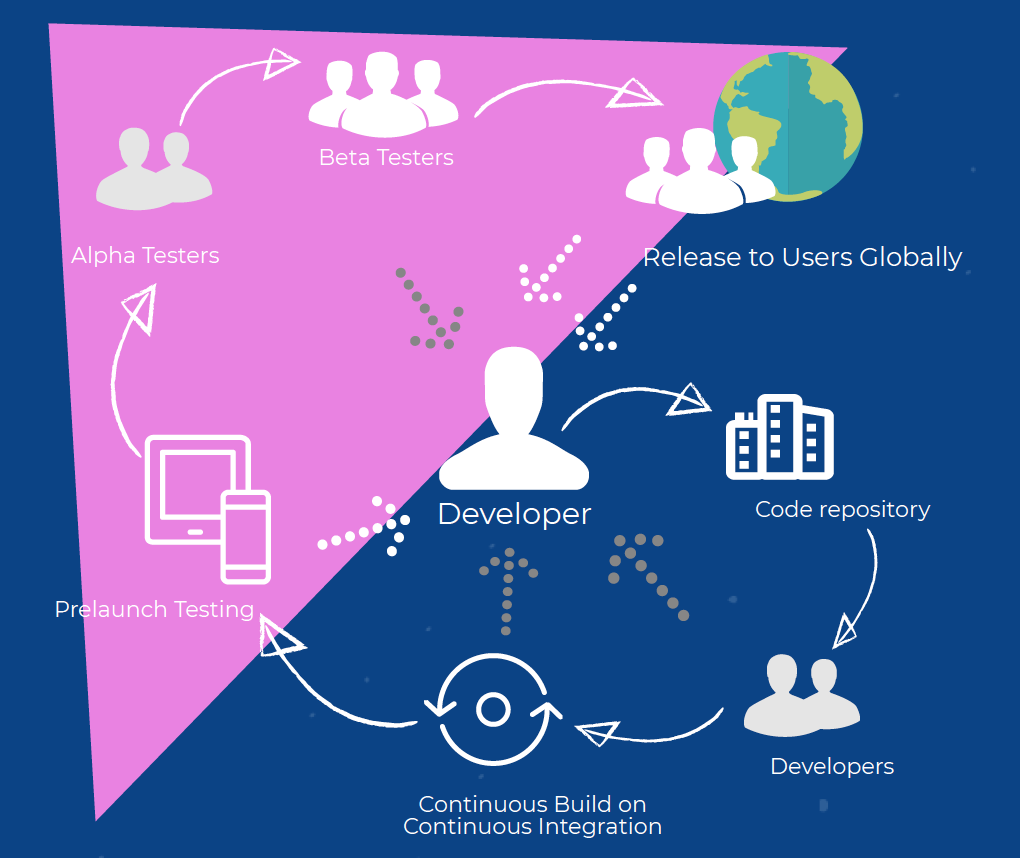
\includegraphics[width=13cm]{images/silvias-developer-centric-figure-mobilesoft2020.png}
    \caption{Sources of feedback for developers}
    \label{fig:sources-of-feedback-for-developers}
\end{figure}

Each source of feedback may stem from humans (for example, in reviews) or from software (for example, from code quality tools such as Lint). This research introduces three sources of software generated feedback.

\subsection{Research Strategy}
The research aims to provide practical and applicable insights to mobile apps developers. As such, the strategy was to predominantly work with development teams for mobile apps to ensure -- as far as practical -- the research is externally validated through their experiences, practices and feedback. As developers need to make choices appropriate to their context the research includes a variety of apps including commercial and not-for profit, small, medium and large development teams and user bases, and has an international flavour with developers situated in various continents including Asia, Europe, and the USA.

As the analytics tools also influence the results the research includes discussions and collaborations with several organisations who create these tools.


\section{My research methodology, and my choices}
As my main research question considers the application of analytics, the research needs to include a combination of usage \& analytics data where the analytics data is then applied with the intent of improving the product quality. The developers may not be successful in achieving improvements, although we hope they will be. They may also be able to improve their practices, so again their current and revised processes are also of interest.

Although I had prior experience in industry of the efficacy and potency of applying usage analytics to improve software development and testing of mobile apps, that experience is generally covered by confidentially agreements, and also the analytics tools have changed and developed markedly since those experiences. Therefore, action research seemed appropriate, particularly as one of the long-term opensource projects had extremely high failure rates according to the de-facto Android analytics tool. I decided it was appropriate and necessary to see if I could directly help that project to improve their mobile apps - \emph{``physician heal thyself"}\footnote{\href{https://en.wikipedia.org/wiki/Physician,\_heal\_thyself}{wikipedia.org/wiki/Physician,\_heal\_thyself}.}.

The next level of validity was that even if this work achieved the desired results, could other development teams achieve similar results by applying a similar approach? To help gain evidence the research engaged a separate opensource development project and development team. 

Working with non-profit opensource projects, where the teams are generally willing to make their practices and results public helps with being able to obtain information and publish the results. However, as many research projects discover, what might work for opensource projects - while important and interesting to the research community - might not matter much to the industry of professional and commercial development teams. 

Opensource apps are a tiny proportion of mobile apps available to users, so another level of learning and validation could be achieved through the insights of these professional and commercial development teams. Surveys tend to have poor response rates and lack the depth or richness I was seeking therefore I chose to engage at a deeper level as a fellow developer interviewing developers of several apps. Of course we would need the permission of their organisations, and some shared examples of their tools, their practices and their results of applying analytics well, and even times when they hadn't.

This research is not immune from also being improved, and similarly the process is likely to have plenty of scope for improvement as we learn more from the various projects, teams, apps, and analytics tools. Similarly, there is scope to find flaws, limitations, and weaknesses in the analytics tools, therefore there was scope in the research to share findings with the teams responsible for these, and related, software tools and to use the experiences and insights from any such sharing as part of this research.

Where practical, triangulation of data and analytics reports was used to help increase the confidence in the analytics and in the efficacy of using mobile analytics. As~\citep{marr2015bigdatabook} recommends:~\emph{``Measure metrics and data backed up or triangulated with other data sources."} and~\emph{``Where possible use a combination of data sets and triangulate the data. In other words, see if each data set delivers the same result so you can confirm and validate the answers."}. Triangulation of research methods is extensively covered in research. For example, \citep{fielding2012_triangulation_and_mixed_methods_designs} provides a rich discussion of triangulation and mixed methods design for various research areas. To the best of my knowledge  %SHOULD-DO decide how much to focus on triangulation, whether to discuss data triangulation as a technique for comparing analytics results (which doesn't seem to quite apply - at least in what I've read).



\begin{comment}
    - Could I try phrasing my RQs as OKRs to see if doing so helps me to improve the clarity and relevance of the RQs.
    - Also, how about creating annotated editions of my RQs where the annotations include context, commentary, connections to other RQs, notes on twitter-style answers to each, etc.
    - We want to know more about 'this' topic. Then provide Operational questions - to be addressed by the research, which will help us learn more about the topic.
    - What's a RQ and what's an analytical lens (to be used to help with the RQ)?
\end{comment}

\section{Research Questions}
\label{section-research-questions}

My research hypothesis is that using mobile analytics can help improve both the work development teams do and the quality of the product they create. Here work includes the development, bug investigation, and testing of the software being created. For the quality of the product I'm focusing on a subset of qualities, which are technology-centric.

The domain of mobile apps was selected for the research as mobile apps are ubiquitous, extremely popular, and have interesting and challenging contexts of use. And within the range of mobile apps the research ended up focusing on Android apps for various reasons including: the analytics tools available, the relative glut of suitable apps available for research, my prior experience and expertise, and their market share.

The core question the research aims to consider is: 
\emph{How can applying analytics improve software development and software testing for mobile apps?}~\label{overall-research-question}
Here the assumption is that analytics can help, as stated by Buse and Zimmermann ~(\citeyear{buse_analytics_2010}); and \emph{``with explicit and implicit feedback now available (almost) continuously, questions arise. How can practitioners use this information and integrate it into their development processes [to decide when to release updates]?"}~\citep{maalej2016_towards_data_driven_requirements_engineering}.

This leads to several related questions that underpin this main question \emph{i.e.}, These are grouped in three categories: sources, value, and impact.

\akb{There are a lot of sub-questions below. You will need to focus on the ones you have data to evaluate, or have more abstract formulations that cover groups of sub-questions.}

\yijun{If possible, you may need to dig out a few MobileSoft research papers to give evidence that these research questions have not been addressed in literature, e.g., \emph{Future Trends in Software Engineering Research for Mobile Apps}~\citep{nagappan2016_future_trends_in_sw_eng_for_mobile_apps}, whether the future work of some paper suggests one does not know the sources, value, or impact of mobile analytics to assess and improve app quality? Is there nothing in the general SE literature studying the "analytics" to "general software quality" problem? If there are such general work, how does "mobile analytics" and "app quality" differentiate the RQs to existing ones...}



\subsection{Sources}~\label{section-sources}
\begin{itemize}
    \item \emph{What sources of analytics are available?} at a superficial level there seem to be those that operate within the app and those that are external to the app, particularly those that gather data at the platform level. Several widespread analytics offerings were evaluated and several more were considered as part of this research and to provide an understanding of the overall context.
    \item \emph{How do the sources that were investigated compare in terms of the data they collect and how they are used?}
\end{itemize}

\subsection{Value}~\label{section-value}
Does using analytics provide quantitative and/or qualitative value that can be measured? Could it provide value in terms of assessing the quality of our work that was invested into developing, testing and preparing software before it was launched?
\begin{itemize}
    \item \emph{How truthy are various analytics offerings?} We discovered numerous errors in various analytics offerings. These results may be of interest to the research community given the endemic nature of mobile analytics in real-world apps in the major app stores.
    \item \emph{How much does the fidelity matter of the analytics offerings?} Can the results be used productively even if they are flawed?
    \item \emph{How does using the various analytics compare with other sources or reflections of software quality?} Research already studies how various sources, such as ratings and reviews, can be used to identify flaws in software. Where and how do analytics fit into the larger context of these tools. \emph{Note: I've not actively compared the sources from a practical perspective, however the Catrobat case-study may be relevant}.
    \item \emph{How can the analytics be used to inform and assess the work that went into creating and testing a particular release?} data from usage analytics can reinforce aspects of what was discovered pre-release (c.f. how Google Android's pre-launch reports cross-identify crashes) it can also identify quality flaws we missed in the development work.
    \item \emph{How can analytics help with bug investigation?} a single bug instance may be hard to assess in terms of the likely scope and impact on a user-base; how, where and when can analytics help with bug investigation? We might also consider practical limits e.g. that are enforced by the real-world analytics we used. 
\end{itemize}

\subsection{Impact}~\label{section-impact}
Here the focus is on whether the value has sufficient impact for anyone else to be interested in using and applying analytics. Given the nature of the research the main measures are practical, \emph{i.e.} in the real-world.
\begin{itemize}
    \item \emph{Do development teams use analytics in their practice?} If development teams find practices useful they will generally try to use them intrinsically. Do they? And if so, how?
    \item It's one thing to be able to improve a measurement such as the crash rate, it's also worth considering whether that has any material impact on other relevant measurements. \emph{Can we discern changes, even improvements, in user satisfaction, retention, etc. through using analytics?} One of the presumptions (identified in research) is that improving quality improves the user's satisfaction with mobile apps. If so, presumably we should be able to measure the effects, even crudely.
    \item \emph{Has anyone else found the work of interest? are there additional evidence of the impact of the work?} Here the main considerations are feedback from other researchers and from Industry e.g. Google.
\end{itemize}



\subsection{On Findings}
\yijun{It will be good to move 1.5 Research Questions here and articulate them as hypothesis or early hypothesis? It is too early to reveal the findings here Maybe you can prepare the reviewers by presenting the findings as confirmation of some "hypothesis", and first discuss about these hypothesis before introducing the facts? }

The research  the hypothesis 



\section{Outline of this thesis}


%%%%%%%%%%%%%%%%%%%%%%%%%%%%%%%%%%
\par\noindent\rule{\textwidth}{0.4pt}
%%%%%%%%%%%%%%%%%%%%%%%%%%%%%%%%%%
\section{The following need relocating}
Bugs are ubiquitous in software (even one of the most respected software engineers, Donald E. Knuth, recognises, publicly acknowledges, \emph{and pays for}~\cite{knuth_trutex, wikipedia__knuth_reward_checks_2020} bugs found in his creations. And self-aware developers expect there will be bugs in their software. \emph{``You are entitled to a reward of at least 0x$1.00 ($2.56) if you are the first person to report a bona-fide error not on those lists."} Donald E. Knuth~\cite{knuth_the_bank_of_san_serriffe}

Even top development teams are likely to learn of bugs they were not able to find, and cannot reproduce. For instance, Google's Android Auto Team have asked for help from end users to identify patterns that may help the team find and address a long-running and frustrating bug in Android Auto~\footnote{\url{https://support.google.com/androidauto/thread/2865341?msgid=44437416}}. As reported by \texttt{autoevolution} in May 2020:  
\emph{"As it turns out, the Android Auto team wasn’t able to reproduce the whole thing, so it’s now asking users to send additional reports with more information to help fix the problem."}~\footnote{~\url{https://www.autoevolution.com/news/google-wants-users-to-help-fix-widespread-android-auto-bug-143760.html}}.

